\chapter{Experiments and results}

\label{ch:Experiments and results}

\setlength{\parindent}{4em}
\setlength{\parskip}{1em}
\renewcommand{\baselinestretch}{1.5}

\section{Hardware for the experiment}

In our project, first we plan how to investigate the EEG data from the subject. There are 2 categories to investigate the data those are software and hardware. When we know like that we go to study how is it different between software and hardware that use in this project and when we already study in it we know that hardware is better than software and we choose it and We plan to design the hardware to use it in experiment.This is materials that we use in our project.

\subsection{EPOC headset by Emotiv}

\subsection{Arduino Uno}

\subsection{Gravitech Gerora WS2812S LED}

\subsection{Visual stimulus (ERP)}
\begin{figure}[ht]
	\centering
	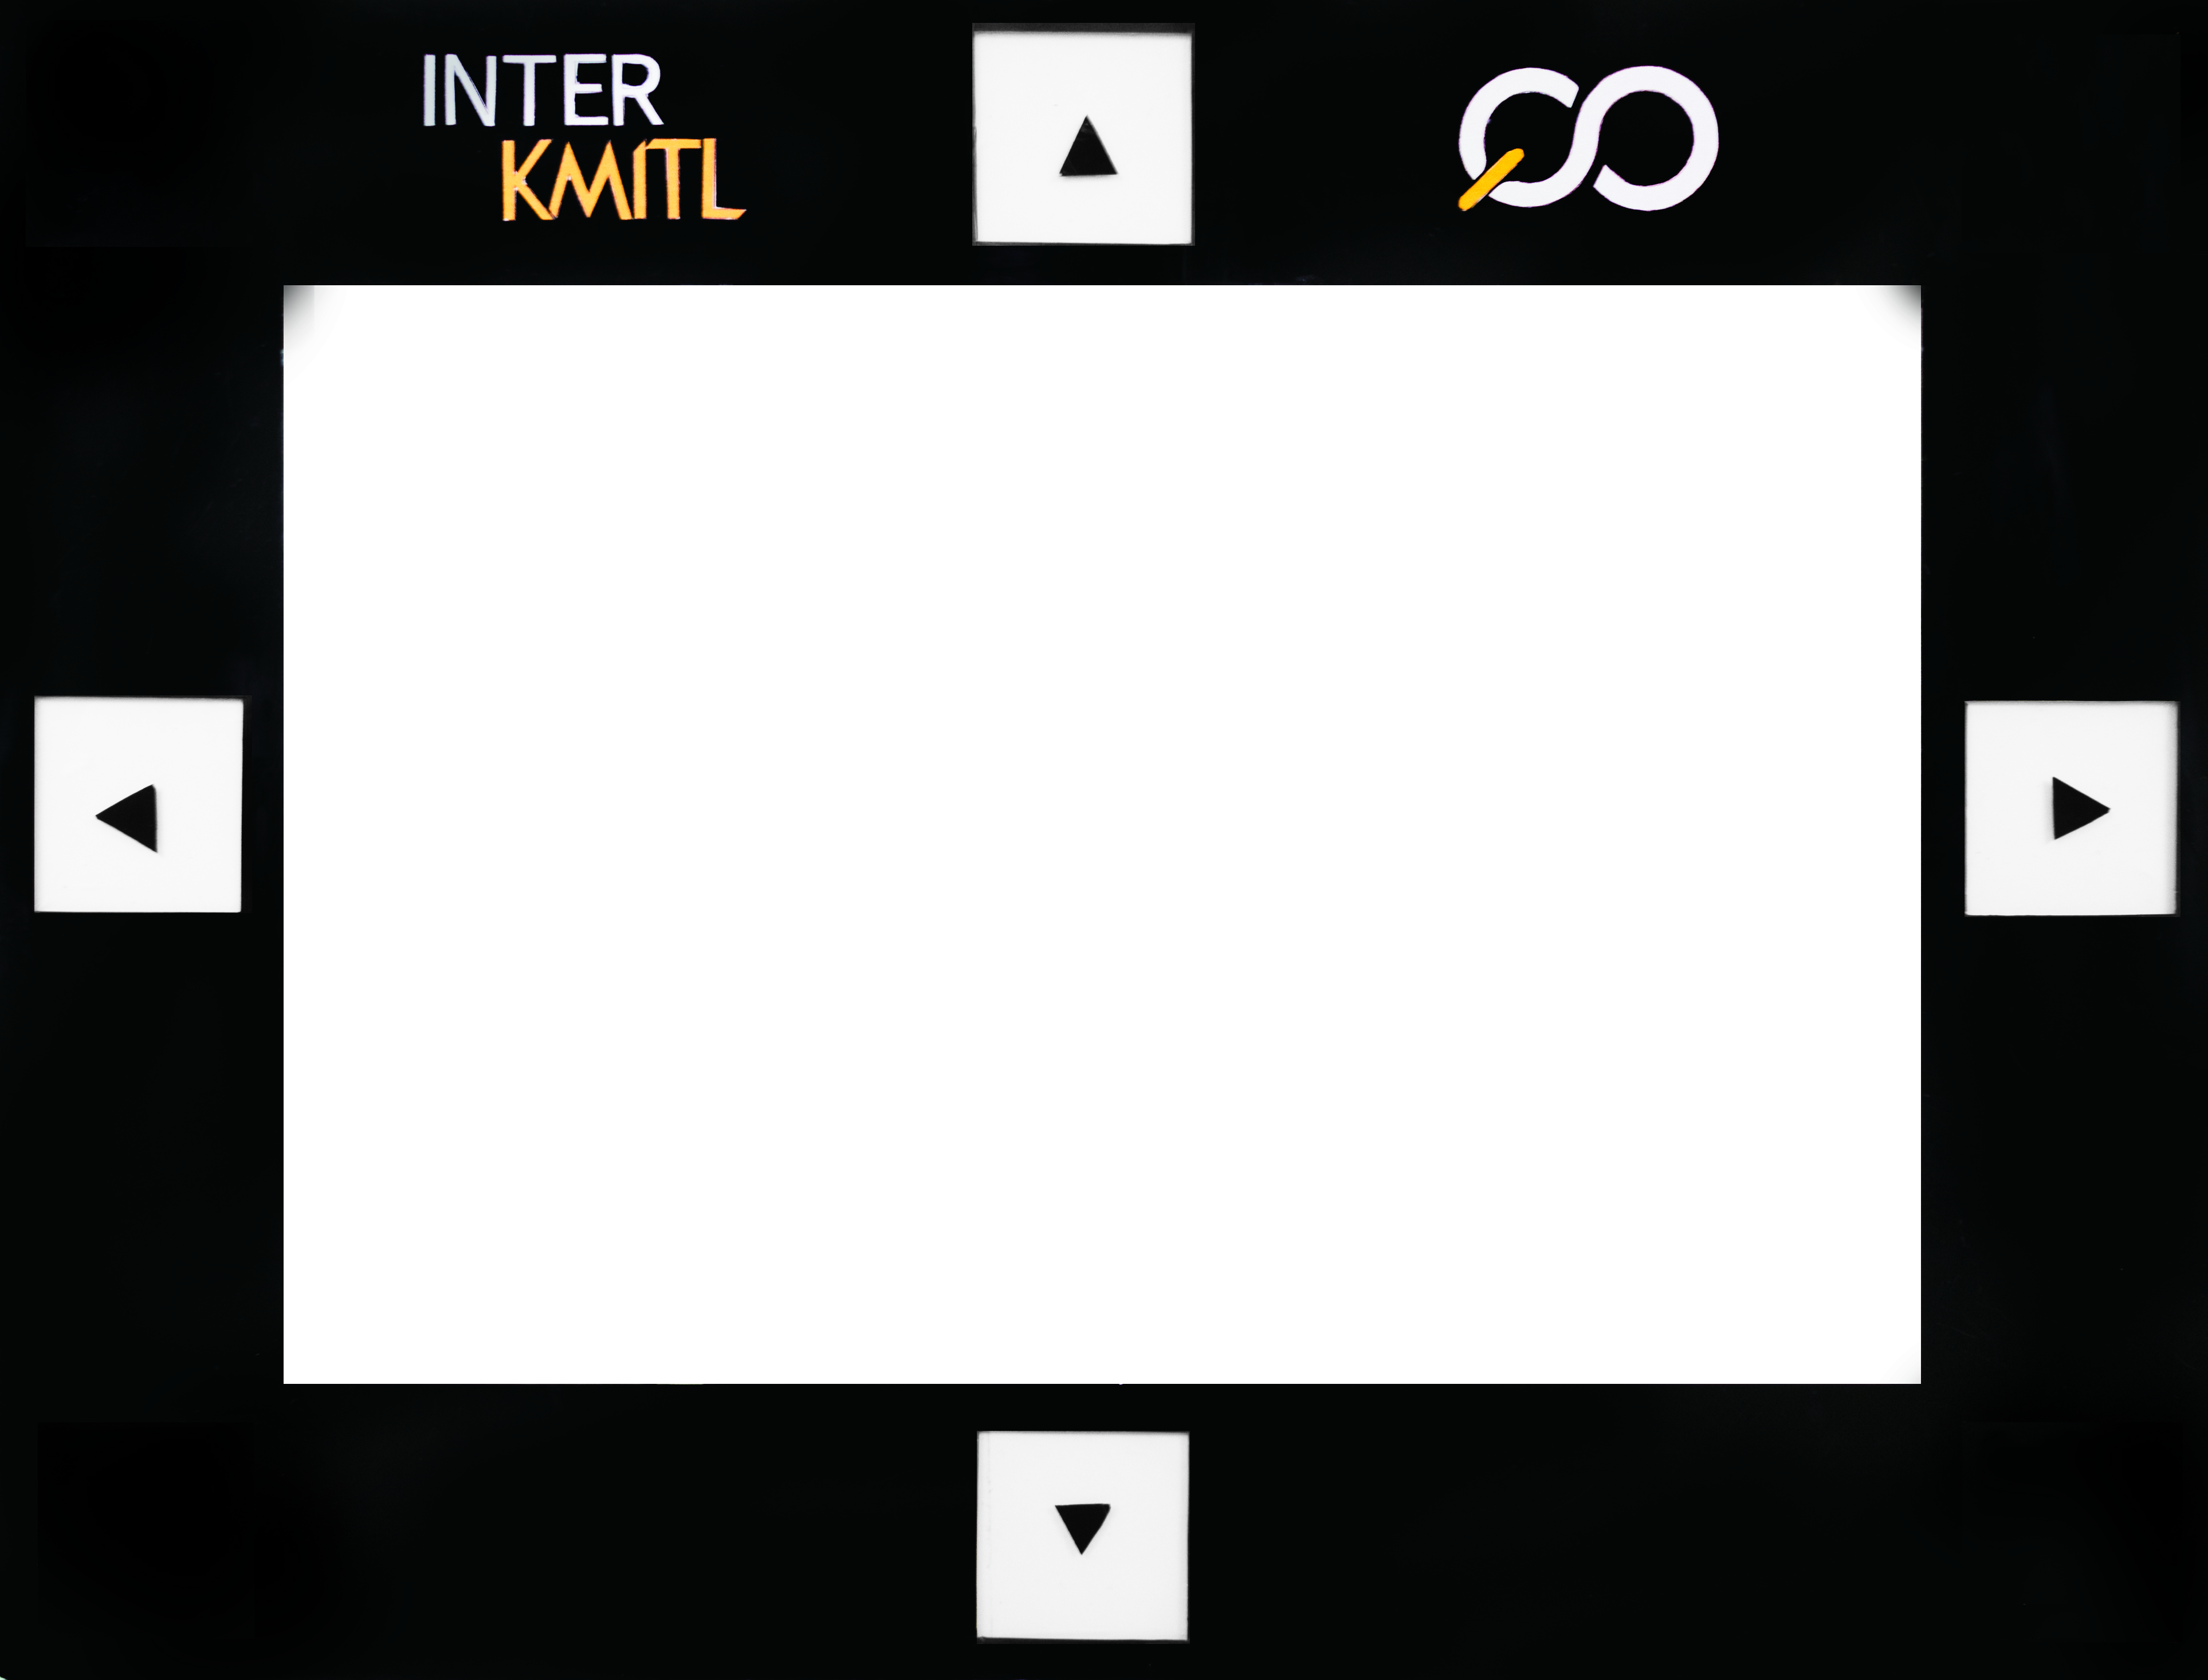
\includegraphics[width=\textwidth]{chapter7/frame_4.jpg}
	\caption{Visual Stimulator}
\end{figure}
\subsection{Visual stimulus (SSVEP)}

\newpage
\section{Experiment I}
\subsection{Experiment Paradigm I}
\begin{itemize}
\item{\textbf{Subjects}}\newline
\hspace{3.0cm}In this experiment, we use 4 subjects. There are SS,OK,WP and NT that is the nickname and firstname of subjects.
\item{\textbf{Stimulus}}
For one trial, we use 11, 15, 19, 23 seconds respectively.
\item{\textbf{Trials}}
We recorded 3, 5, 7, 9 times for each set of parameter.
\item{\textbf{Environment}}
In this experiment, we control the light illuminate value at 37 Lux.
\item{\textbf{Parameters}}\\
There are 4 parameters. First is flickering type, stimulus, sample length and epoch time.
\end{itemize}

\newcolumntype{P}[1]{>{\centering\arraybackslash}p{#1}}
\begin{table}[ht]
\centering
\begin{tabular}{| P{.3\linewidth} | P{.3\linewidth} | P{.3\linewidth} |}
			
			\hline 
			\textbf{Parameter} & \textbf{Experiment1}  & \textbf{Experiment2}\\
			\hline 
			Flickering type & Regular & Uniform random   \\
			\hline 
			Stimulus & \multicolumn{2}{c}{Modular} \vline\\
			\hline 
			Sample Length & \multicolumn{2}{c}{64samples/epoch} \vline\\
			\hline 
			Epoch time & \multicolumn{2}{c}{500 ms} \vline\\
			\hline
		\end{tabular}       
\caption{Experiment paradigm}
\label{table:2}
\end{table}

\begin{figure}[ht]
	\centering
	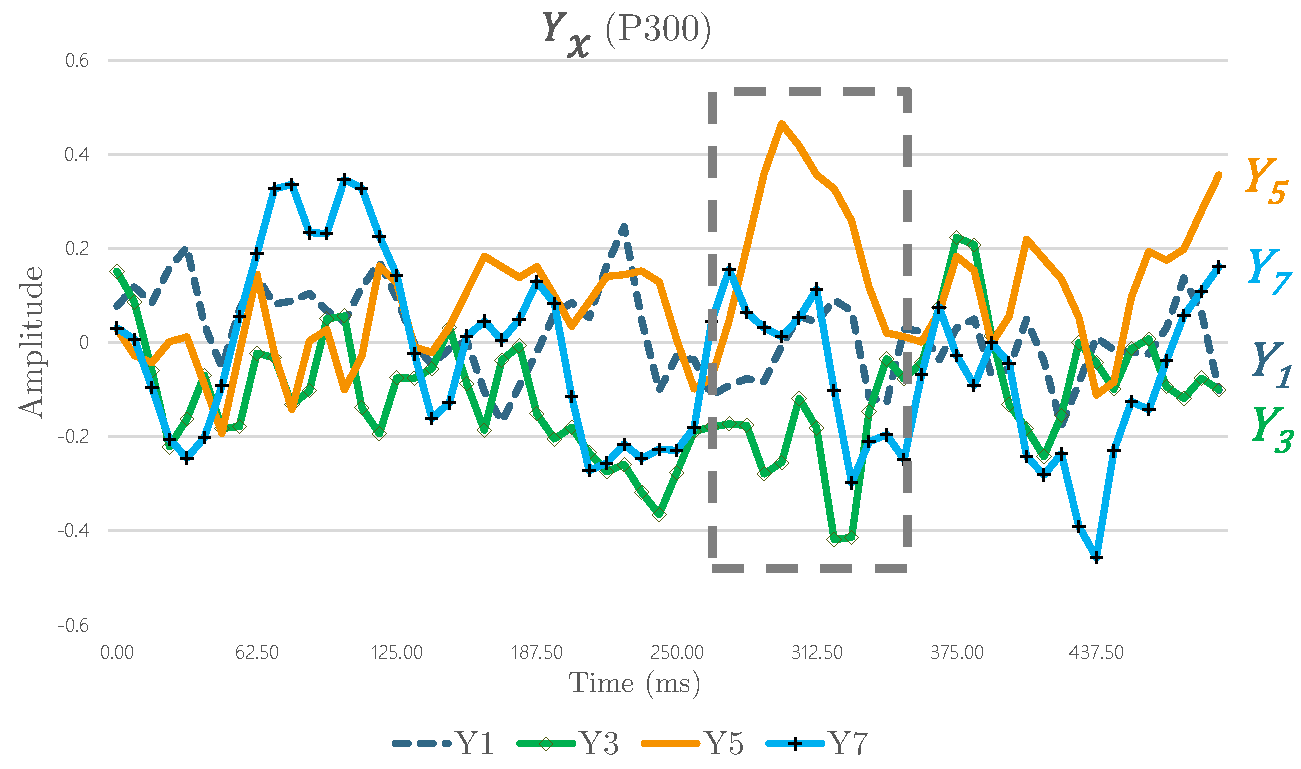
\includegraphics[width=\textwidth]{chapter7/erp_result.pdf}
	\caption{}
\end{figure}

\subsection{Experiment result I}
\begin{figure}[ht]
	\centering
	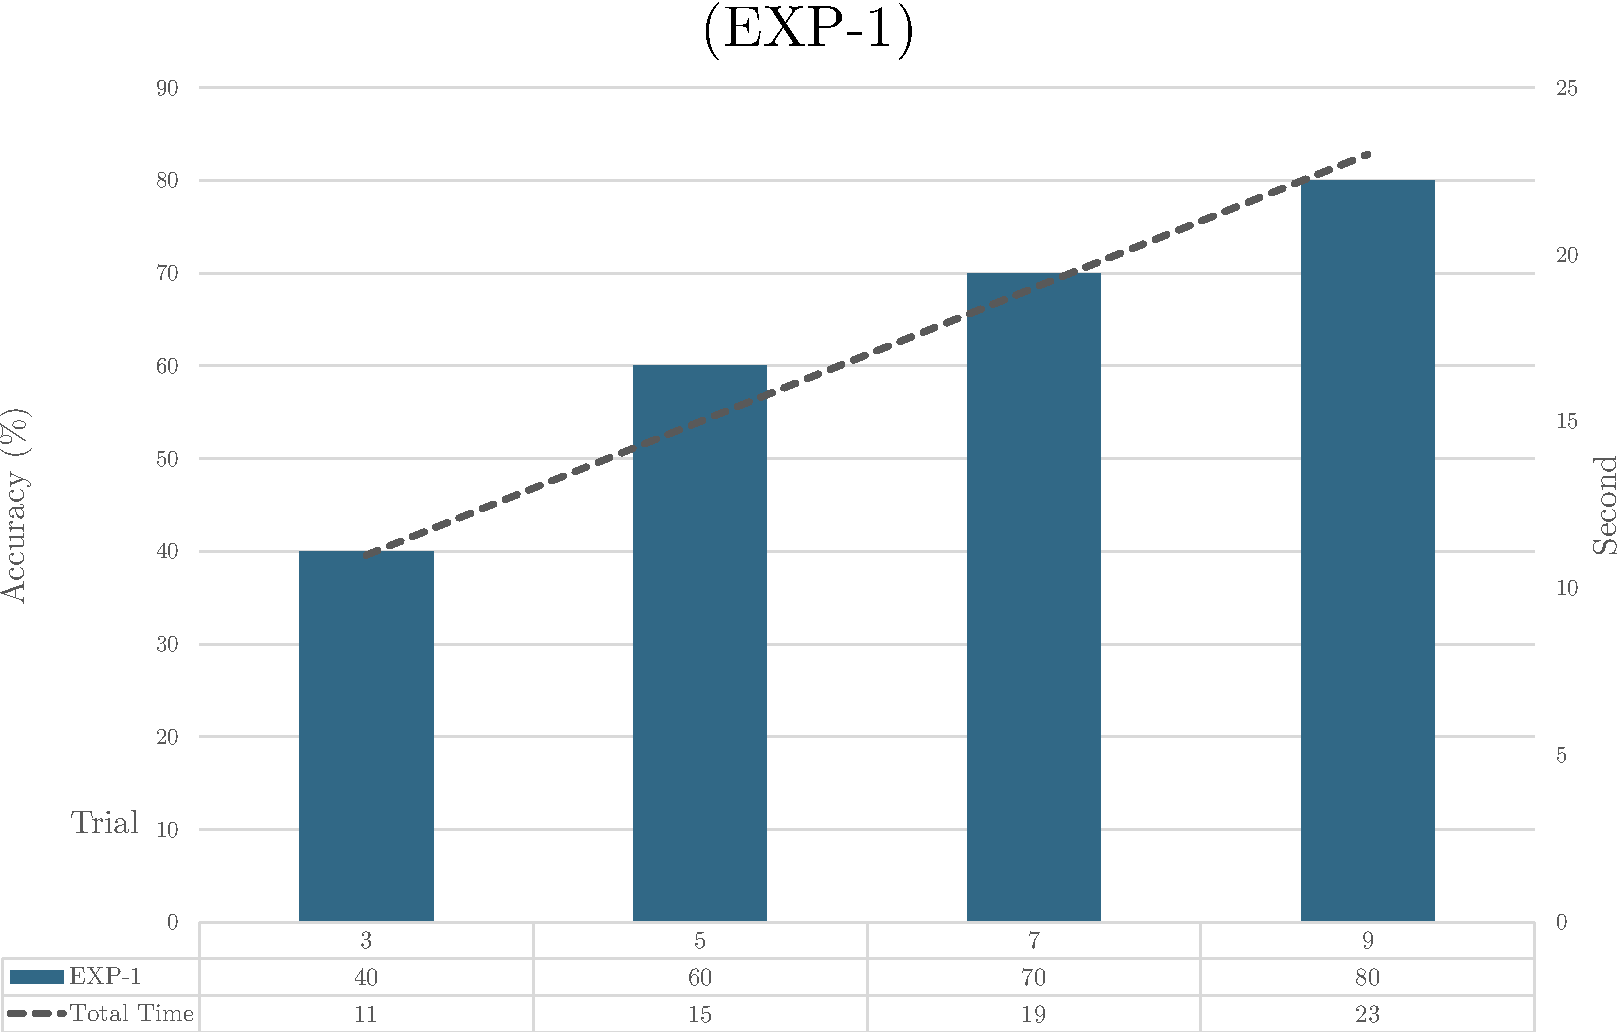
\includegraphics[width=\textwidth]{chapter7/result_1.pdf}
	\caption{Result of experiment1}
\end{figure}

\begin{figure}[ht]
	\centering
	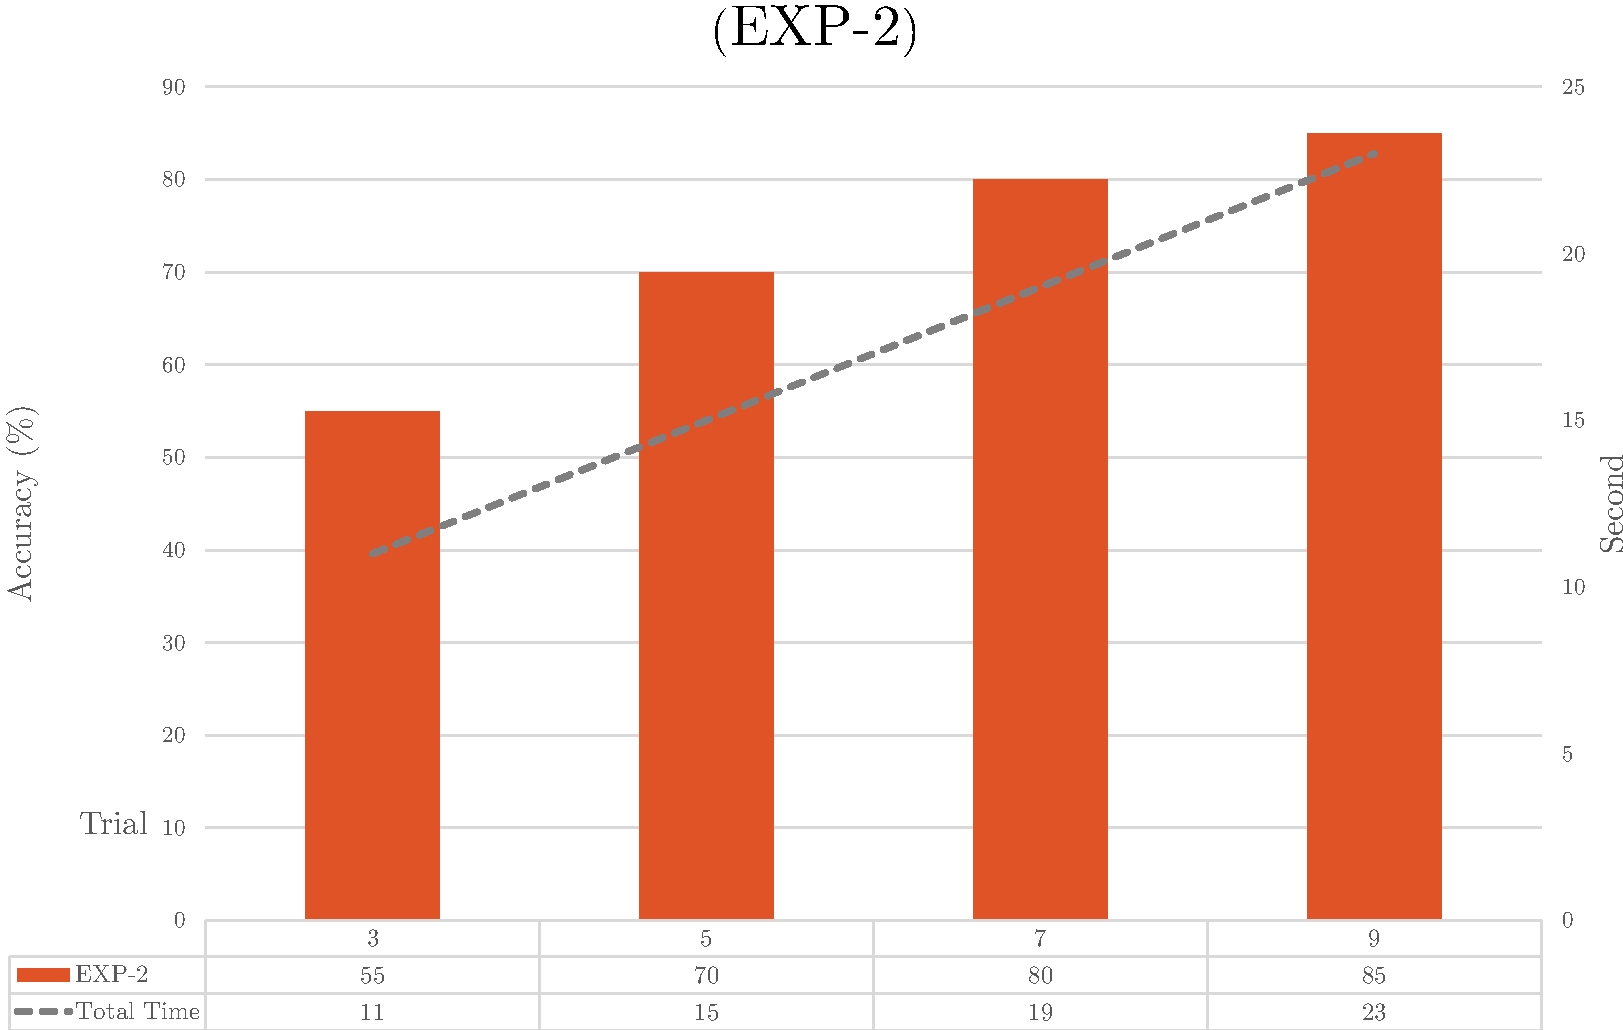
\includegraphics[width=\textwidth]{chapter7/result_2.pdf}
	\caption{Result of experiment2}
\end{figure}

\begin{figure}[ht]
	\centering
	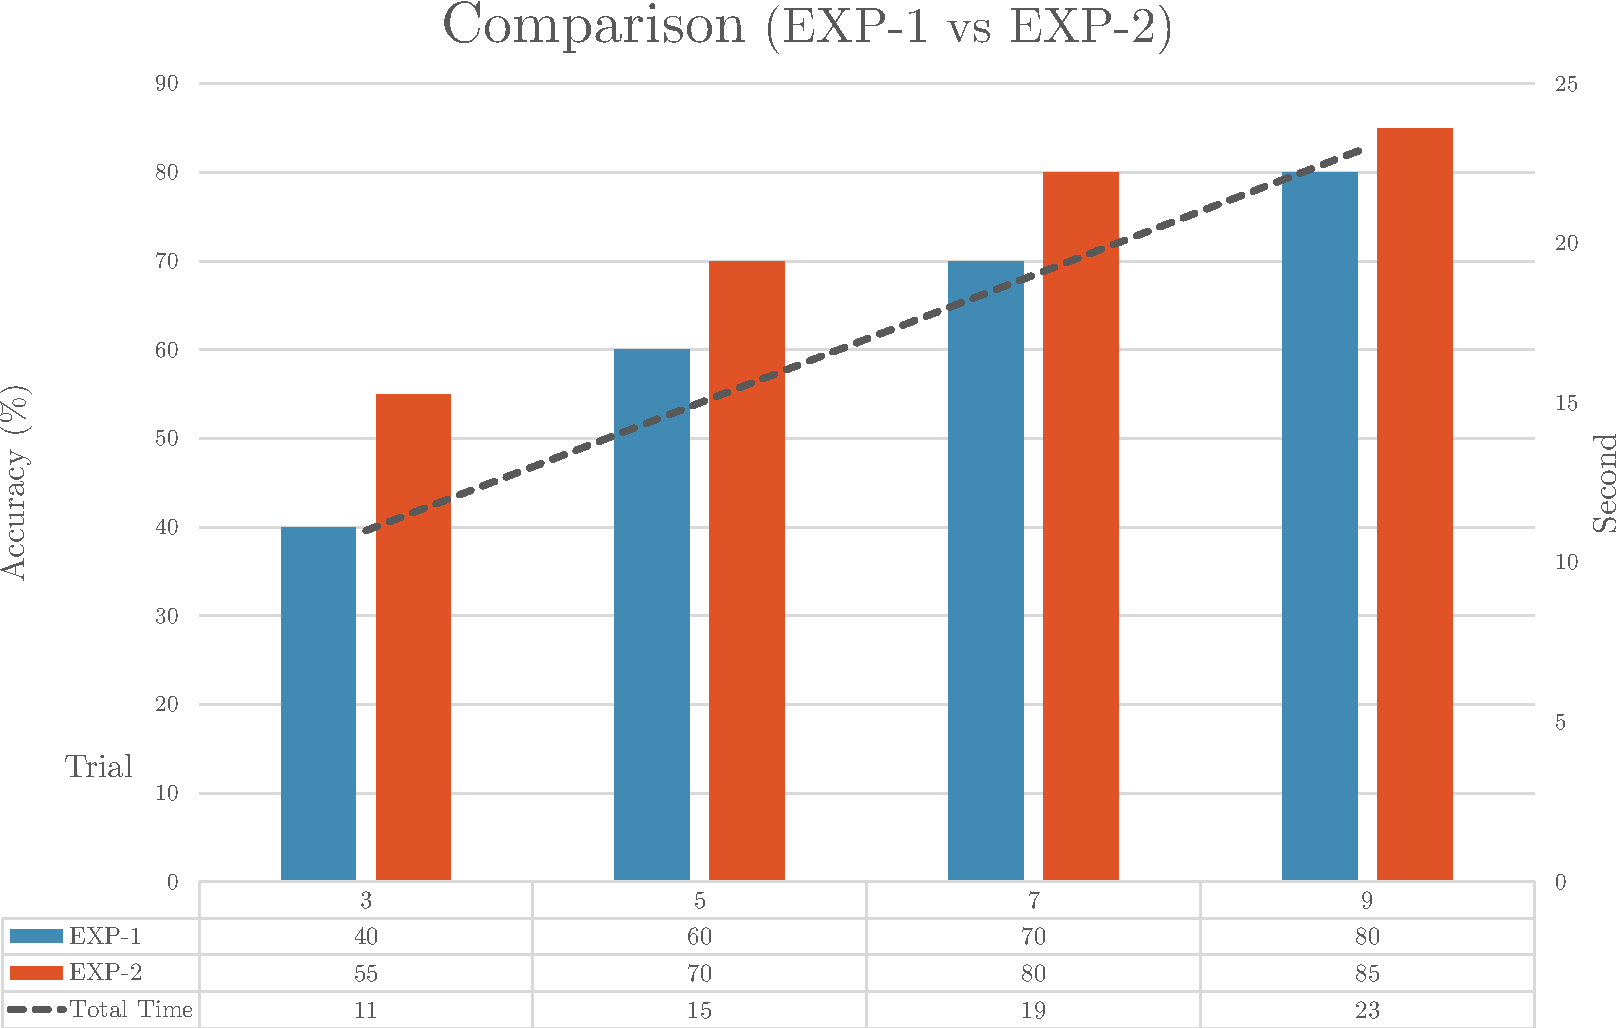
\includegraphics[width=\textwidth]{chapter7/result_12.pdf}
	\caption{Comparison between the result of experiment1 and 2}
\end{figure}

\begin{table}[ht]
\centering
\resizebox{\textwidth}{!}{
\begin{tabular}{| c | c | c | c | c |}

			\hline 
			\multirow{2}{*}{\textbf{Trial(time)}} & 
  			\multirow{2}{*}{\textbf{Total time(sec)}}  & 
            \multirow{2}{*}{\textbf{Subject}} &
            \multicolumn{2}{c|}{\textbf{Accuracy of flickering type}} \\
            \cline{4-5}
            &&&\multicolumn{1}{c|}{\textbf{Regular}} &\multicolumn{1}{c|}{\textbf{Uniform}}  \\
			\hline 
			\multirow{4}{*}{3}&\multirow{4}{*}{11}&OK&30&60 \\
			\cline{3-5}
			&&WT&50&65 \\ \cline{3-5}
			&&SS&45&50 \\ \cline{3-5}
			&&NT&35&45 \\
            \hline
			\multirow{4}{*}{5}&\multirow{4}{*}{15}&OK&55&75 \\
			\cline{3-5}
			&&WT&60&70 \\ \cline{3-5}
			&&SS&65&70 \\ \cline{3-5}
			&&NT&60&65 \\
            \hline
            \multirow{4}{*}{7}&\multirow{4}{*}{19}&OK&70&75 \\
			\cline{3-5}
			&&WT&80&80 \\ \cline{3-5}
			&&SS&65&85 \\ \cline{3-5}
			&&NT&65&80 \\
            \hline 
            \multirow{4}{*}{9}&\multirow{4}{*}{23}&OK&85& \\
			\cline{3-5}
			&&WT&& \\ \cline{3-5}
			&&SS&& \\ \cline{3-5}
			&&NT&& \\
            \hline 
		\end{tabular}       
        }
\caption{Experiment result}
\label{table:3}
\end{table}

\newpage
\section{Experiment II}

























